\label{key}\documentclass[letterpaper, 12pt,oneside]{article}
\usepackage{amsmath}
\usepackage{graphicx}
\usepackage{xcolor}
\graphicspath{{Imagenes/}}
\usepackage[utf8]{inputenc}
\usepackage{listings}
\usepackage[hidelinks]{hyperref}

\title{\Huge Taller de Herramientas Computacionales}
\author{Josué Artemio Hernández Rodríguez}
\date{24/Enero/2019}

\begin{document}
	\maketitle
	\begin{center}
		
\includegraphics[scale=0.7]{3.jpg}
	\end{center}

	\newpage
	
	\title{\huge \textit{Bitacora problema 1 }}\\
	El problema consiste en calcular el máximo común divisor de dos números, lo que hice fue usar el condicional while b > 0: el resto pasa a ser b, luego esa misma b es igual al modulo de a y b(resto), y si es ese el numero mayor que divide a ambos con cero como resto, ese es el mcd.
	
	\begin{figure}[h]
		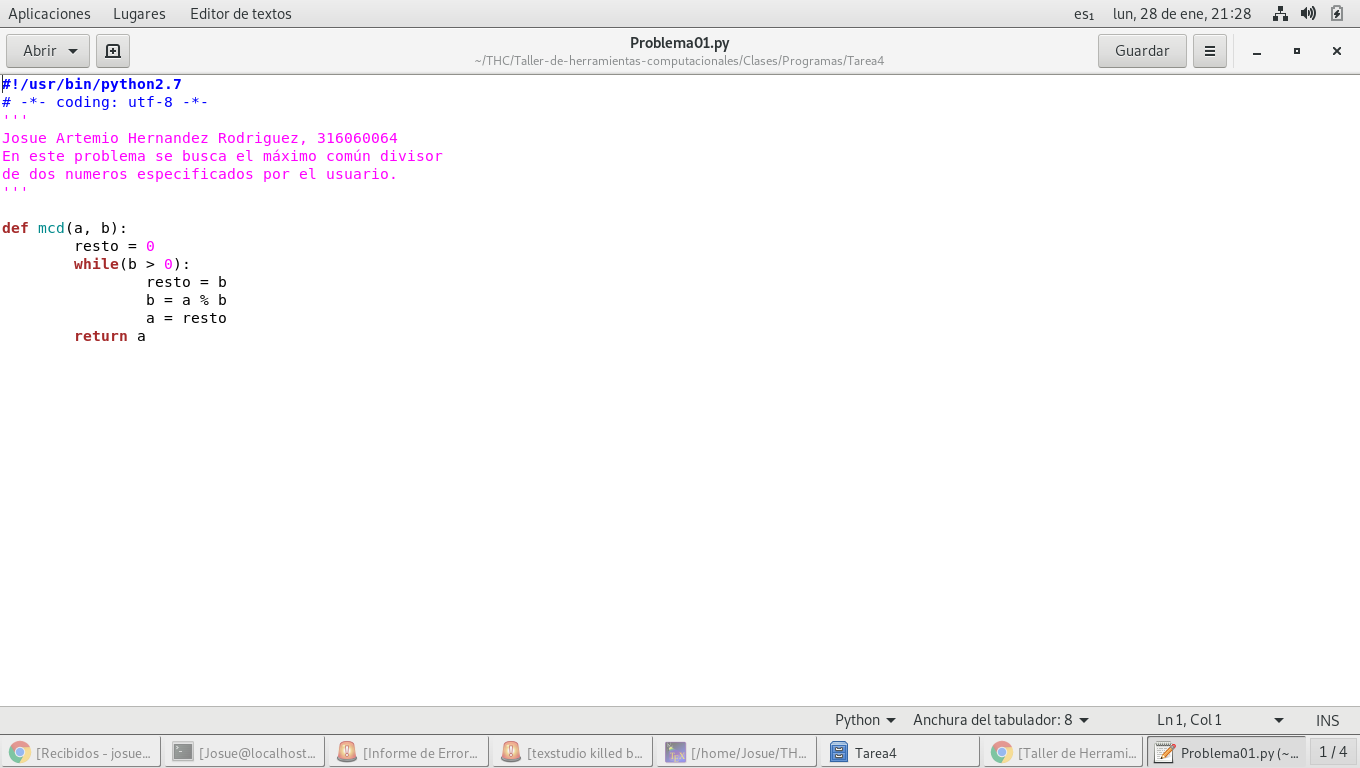
\includegraphics[scale=0.3]{pro01.png}
	\end{figure}

	
	
	
	
	
	
	
	
	
	
	
	
\end{document}
